\section{Testing and continuous integration} 
\label{sec:tests}

\begin{figure}[h!]
  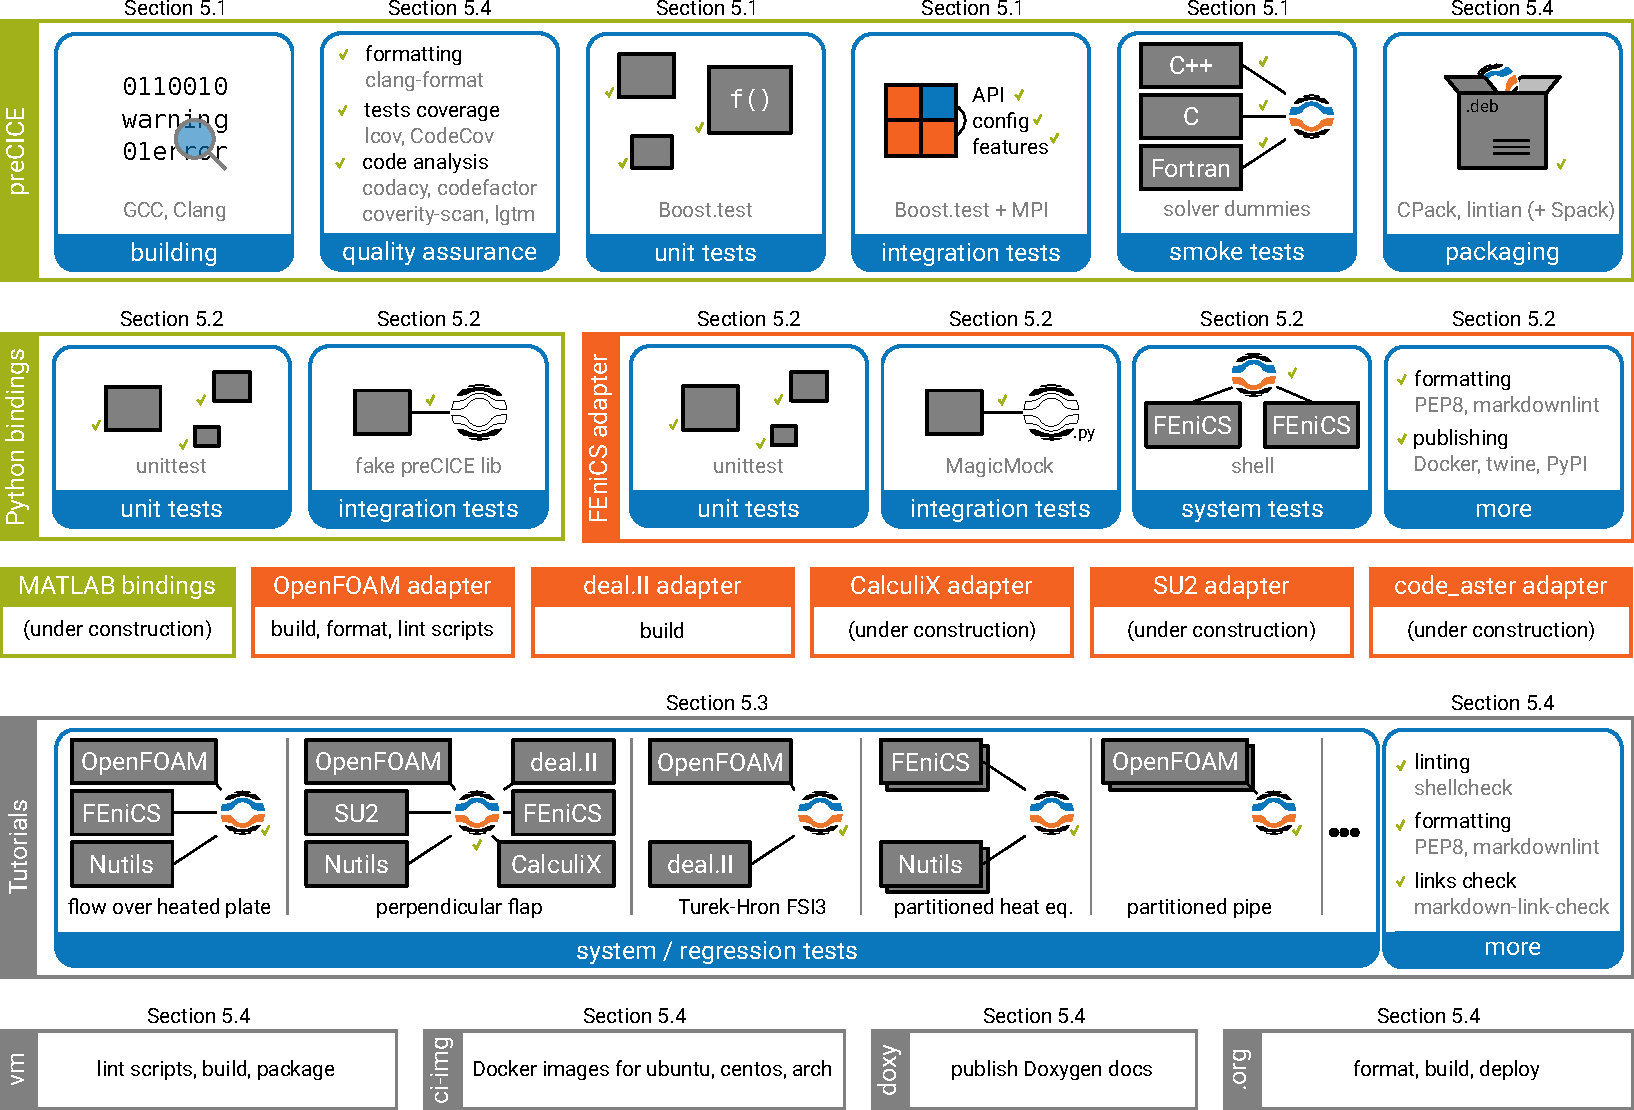
\includegraphics[width=\textwidth]{figs/tests-overview.pdf}
  \caption{Overview of the testing and continuous integration workflows for different preCICE components.
  Each box represents a separate project repository. The non-native language bindings depend on preCICE.
  The adapters depend on language bindings or directly on preCICE.
  The tutorials and system tests depend on all the adapters.
  The components at the bottom-most row (virtual machine image, CI images, Doxygen documentation, website) depend on one or more other components.
  Read more details about each workflow in the section number listed above it.}
  \label{fig:tests-overview}
\end{figure}

The core preCICE library and the non-core components are developed in separate repositories,
each with a number of continuous integration (CI) workflows. These workflows are tests, quality assurance checks,
or operations to prepare and validate packages. We find such workflows to be indispensable for multi-component,
multi-developers projects, as they answer questions such as
``will the code still compile and behave in the same way if we integrate these changes?'',
``will a simulation still give the same results?'', and ``will these changes have side-effects in other (potentially not regularly updated) components?''.
In other words, these workflows facilitate further development by ensuring that everything still works.

Figure~\ref{fig:tests-overview} depicts the currently deployed workflows.
As one may observe, the granularity of testing and CI correlates to the
number of users and developers involved in each subproject.
In some cases, it may also be enabled or hindered by the respective programming language environment.
As the most important and actively developed component, the core library is rigorously tested in a wide range of levels.
The rich tooling collection of Python enables the CI of the Python bindings and the FEniCS adapter,
while we are gradually adding similar workflows to the rest of the adapters.
The tutorials provide a platform to test every component in complete simulations (system tests with results regression checks).
Finally, a few additional workflows keep non-critical systems up-to-date.

The number and diversity of components required to construct a complete coupled simulation
(at least two participants + multiple components per participant), as well as the challenges in
testing each component in isolation, makes testing a coupling library significantly more complex than testing a linear algebra solver library, for example.
Complex testing approaches of significant novelty are required.
We structure the rest of the section following the different complexity levels.
In \autoref{ssec:unit_and_integration_tests_preCICE}, we present the CI of the core library, for which
no interaction with other components is required and the respective runtime is relatively short.
In \autoref{ssec:unit_and_integration_tests_other}, we continue with the CI of non-native language bindings and adapters. This layer depends on
the core library, as well as on external components (the solvers), leading to a need for testing in isolation.
In \autoref{ssec:system_tests}, we construct system tests for the complete software stack.
Finally, in \autoref{ssec:additional_checks}, we give an overview of additional checks and workflows which we use across the whole project.

\subsection{Tests for the preCICE core library}
\label{ssec:unit_and_integration_tests_preCICE}

To test the complete functionality of the preCICE core library, heterogeneous test setups are needed.
Individual tests may require one or more logical participants running on one or more MPI ranks. 
To solve this intrinsic problem of testing a communication and orchestration library in a parallel environment, the core library tests are run on 4 MPI ranks.
Partitioning these 4 ranks allows to cover various scenarios, from testing math functions on a single rank, over testing parallel mappings on 3 ranks, up to testing scenarios with a serial participant on a single rank coupled to a parallel participant on 3 ranks.
% The test framework
As mature MPI-aware testing frameworks are not available, we developed our own testing framework extending \incode{Boost.test} to support the aforementioned criteria.

The extension of \incode{Boost.Test} provides a custom domain-specific language (DSL), which is used to set up a \incode{PRECICE_TEST()}.%, which allows to specify named logical participants running on a given amount of ranks alongside local and global setup requirements.
The DSL specifies the name of local participants used in the test, followed by the amount of ranks and optional requirements.
If a test contains only a single participant, then its name can be omitted.
The DSL is human-readable, examples are \incode{"A"_on(2_ranks), "B"_on(1_rank)} or simply \incode{1_rank}.
The implementation of the DSL firstly restricts the MPI communicator size to the required amount of total ranks, followed by grouping ranks by name, forming communicators for the logical participants.
Further specified requirements on logical participants, such as initialization of sub-components, are then handled inside the isolated state of each participant.
The result of each \incode{PRECICE_TEST()} is an immutable object which, for each test rank, provides access to the context including name and communicator information of the local participant.
The \incode{context} holds further information about the setup, information which allows to sanitize user input provided to utility functions.
At the end of each test, the context object firstly reverts all changes made by setup requirements, secondly ungroups the communicators, and finally synchronizes all ranks, including ranks not needed by the test.
See \autoref{fig:testdsl} for example configurations of this framework.


\begin{figure}[h!]
  \centering
  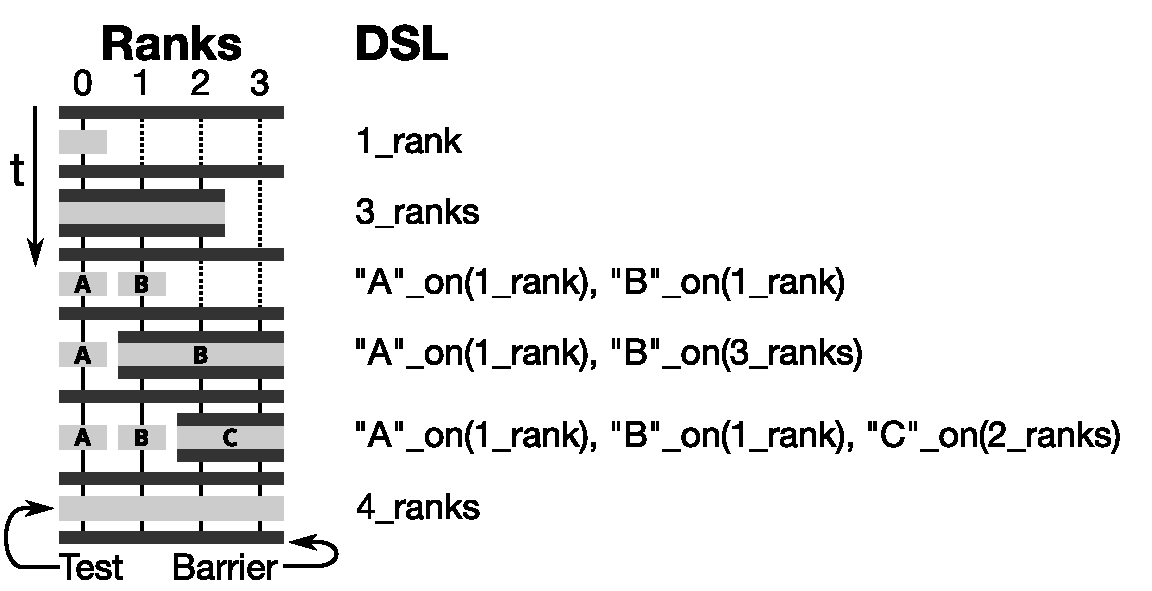
\includegraphics[width=0.75\textwidth]{figs/tests-dsl}
  \caption{%
    This figure depicts the MPI communicator setup on the left corresponding to a sequence of test setups on the right.
    The testing framework uses 4 MPI ranks, depicted by the vertical lines.
    Horizontal black bars are barriers and dotted lines are ranks which are unused during a test setup and hence idle.
%
    Each test starts with \incode{PRECICE_TEST(...)}, containing an expression based on the DSL, which results in a complete test setup.
    The test DSL specifies the name of local participants followed by the amount of ranks.
    The name is optional for tests containing only a single participant.
  }
  \label{fig:testdsl}
\end{figure}

The core library tests can be categorized into unit tests, integration tests, and code-example tests.
Currently, preCICE is tested with a total of 438 unit and integration tests.

% Unit tests
\paragraph{Unit tests} This type tests a component in isolation, using its public interface.
The test functions manually setup the majority of required components and partition the available ranks according to the needs of the test.
% Such unit tests can be classified further by the partitioning of required ranks:
The needs for partitioning vary:
First, many unit tests handling geometric functions, VTK exports, and mesh internals require only a single logical participant and run on a single rank.
Furthermore, components such as VTK exports and radial-basis-function mappings have additional functionality when running in parallel, hence require multiple ranks on a single logical unit.
Finally, inter-code communication, the coupling schemes, and the mesh partitioning require multiple logical participants.
Each of these logical participants may run on one or multiple ranks.
See \autoref{lst:example-unit-test} for an example of a unit test.

\begin{listing}[h!]
  \centering
\begin{minipage}{0.85\linewidth}
\begin{minted}[linenos,numbersep=5pt,gobble=0,frame=none,framesep=0mm]{cpp}
BOOST_AUTO_TEST_CASE(ParallelMappingTest)
{
  PRECICE_TEST(""_on(4_ranks).setupMasterSlaves(), Require::PETSc);
  constexpr int dims = 2;
  // Setup InMesh
  mesh::PtrMesh inMesh(new mesh::Mesh("InMesh", dims));
  mesh::PtrData inData = inMesh->createData("InData", dims);
  getDistributedInMesh(context, inMesh, inData);
  // Setup OutMesh ...
  // Setup Mapping
  PetRadialBasisFctMapping<Gaussian> mapping{
      Mapping::CONSISTENT, dims, Gaussian{5.0}};
  mapping.setMeshes(inMesh, outMesh);
  // Test the Mapping preparation
  BOOST_TEST(not mapping.hasComputedMapping());
  mapping.computeMapping();
  BOOST_TEST(mapping.hasComputedMapping());
  // Test the Data Mapping
  BOOST_TEST(not mapping.hasComputedMapping());
  mapping.map(inData->getID(), outData->getID());
  BOOST_TEST(outData->values() == expectedData);
}
\end{minted}
\end{minipage}
\caption{%
Example unit test of a parallel RBF mapping running on 4 ranks.
Further requirements on the test are the setup of the master-slave communication and the initialization of PETSc.
First the test defines meshes and associated data followed by setting up and executing the mapping.
The result is the checked against the expected outcome.
The example showcases the preparation involved in testing individual components of preCICE in a parallel context.
}
\label{lst:example-unit-test}
\end{listing}

% Integration tests
\paragraph{Integration tests} This type uses the API of preCICE itself to test specific scenarios, hence the test setup is handled using a preCICE configuration file.
Individual logical participants may run on a single rank each to test
% one/two/three-way
coupling of serial solvers with various setups.
Another very common setup consists of two logical participants running on two ranks each.
This allows to thoroughly test the partitioning behavior given various mapping schemes.
Integration tests are also used to reproduce and fix bugs reported by users.
See \autoref{lst:example-integration-test} for an example of an integration test.

\begin{listing}[h!]
\begin{minted}[linenos,numbersep=5pt,gobble=0,frame=none,framesep=20mm]{cpp}
BOOST_AUTO_TEST_CASE(ParallelIntegrationTest2x2)
{
  PRECICE_TEST("SolverOne"_on(2_ranks), "SolverTwo"_on(2_ranks));
  std::string meshName, writeDataName, readDataName;
  if (context.isNamed("SolverOne")) {
    meshName      = "MeshOne";
    writeDataName = "Data1";
    readDataName  = "Data2";
  } else {
    // ...
  }
  SolverInterface interface(context.name, _pathToTests + "test-config.xml",
      context.rank, context.size);
  // set mesh vertices and initialize
  std::array<double, 4> inValues, outValues;
  while (interface.isCouplingOngoing()) {
    interface.readBlockScalarData(readDataID, 4, vertexIDs, inValues);
    if (context.isNamed("SolverOne")) {
      outValues = inValues;
    } else {
      outValues = solveSystem(inValues);
    }
    interface.writeBlockScalarData(writeDataID, 4, vertexIDs, outValues);
    interface.advance(1.0);
  }
  BOOST_TEST(outValues == expectedValues);
}
\end{minted}
\caption{%
  Example integration test involving two parallel participants \incode{SolverOne} and \incode{SolverTwo} running on two ranks each.
  The \incode{context} object provides information about the identity of the current rank.
  This information is used to setup further local information such as mesh and data names.
  Integration tests then directly construct a \incode{SolverInterface} and use preCICE API calls to run the test.
}
\label{lst:example-integration-test}
\end{listing}

% Code-example tests
\paragraph{Code-example tests} This type smoke-tests native bindings using the provided examples.
Native-bindings are C and Fortran bindings, which are implemented using the C++ API of preCICE and linked directly into the library.
Non-native bindings such as Python are covered in \autoref{ssec:unit_and_integration_tests_other}.
Each language binding comes with an example program called a \emph{solverdummy}. All solverdummies implement the same functionality and provide a template for using the preCICE API in the respective programming language.
The code-example tests themselves consist of three steps:
First, the tests build each solverdummy and link it to the preCICE library. This tests a common subset of the interface of the bindings for completeness and assures that the build system is functional.
Second, they run a small coupled simulation coupling each solverdummy to itself. This ensures that the used language binding is working correctly.
Finally, they run a small coupled simulation coupling different solverdummies to each other. This ensures that the bindings (of different languages) are compatible.

\subsection{Tests for adapters and bindings}
% Old title Unit and Integration Tests for Adapters and Non-Native Bindings
\label{ssec:unit_and_integration_tests_other}

As explained in \autoref{ssec:building} and \autoref{sec:adapters}, language bindings and adapters are organized in independent repositories. The requirements for tests of such non-core components are identical to the ones for the core library: the non-core components must also comprise of valid code, their individual units should behave in the correct way and work together, while continuous integration tests should be performed on every commit to each component repository. We again distinguish unit tests and integration tests.

\paragraph{Unit tests} We do not need a special treatment for unit tests of non-core components. Note that non-core components are written in various languages. This requires the use of suitable testing frameworks for each language, such as the Python module \inpython{unittest} for the Python bindings and the FEniCS adapter.

\paragraph{Integration tests} Non-core components use preCICE through its API, treating it as a regular, black-box dependency. This safeguards low software coupling, but also leads to a technical complication as already mentioned above: Due to the very nature of coupled simulations, preCICE requires at least two participants for executing most steps of a simulation. This cannot be avoided easily (since the components are not able to modify preCICE itself) and, therefore, it is not trivial to test each component independently.

To solve this problem we use a strategy commonly known as \emph{mocking}. This is a well-known and widely established software engineering practice~\cite{fowler2007mocks}, but not as widespread in the scientific software community. Mocking is useful, if the system under test (non-core component) has another component (preCICE) as a dependency and interacts with this component through its API. Since we want to avoid starting a second participant in our integration tests, we use a mocked version of preCICE instead of the original one. This mocked preCICE returns fake output for testing and does not rely on any other components.
In the following, we give two examples for our implementation of this testing pattern: first, integration tests in the FEniCS adapter and, second, integration tests in the Python language bindings of preCICE. In both cases, API calls to the fake version of preCICE do not require any initialization of a second participant and hard-coded fake values are returned. This allows to write short and simple tests.

Mock testing for the FEniCS adapter heavily relies on the Python module \inpython{unittest.mock}, which allows to create a \inpython{MagicMock} object that is used to provide a fake implementation of functions or objects. Additionally, the module provides a \inpython{patch} function that allows to replace a module that a test imports with a fake version of the same module, at runtime. These two pieces allow us to replace the Python bindings of preCICE with a fake version. For a detailed example, please refer to~\cite{rodenberg2021fenicsprecice}.

Mock testing for the Python bindings is more involved, since the bindings rely on two different languages, C++ and Python, and (to the authors' knowledge) no mocking framework exists for this purpose. We, thus, test the Python bindings by building a specific executable, where we link against the mocked version of preCICE: a single \inbash{SolverInterface.cpp} with a fake implementation. We do include the original interface of preCICE (\inbash{SolverInterface.hpp}) to make sure that the API is consistent. This allows us to keep the application code of the Python bindings clean and to decide whether we want to use the real or fake implementation of the preCICE library at compile time.
The integration tests of the Python bindings then allow us to check for the correctness of type conversions done by the language bindings, such as converting a C++ \incode{double*} array to a numpy array~\cite{NumPy} using Cython~\cite{behnel2011cython}. An example is given in \autoref{lst:setMeshVertices}).
Our mocking approach leads to a non-standard \inpython{setup.py} build script, which allows us to choose whether we want to build the real executable or the one intended for testing through the standard interface of \inpython{setuptools}\footnote{\inbash{python3 setup.py install} or \inbash{python3 setup.py test}}. A nice side effect of this testing pattern is that preCICE itself is not even needed and does not have to be installed on the system running the tests.

\begin{listing}[h!]
\begin{minted}{cpp}
void setMeshVertices(int meshID, int size, const double *positions, int * ids){
  std::vector<int> fake_ids = get_hardcoded_ids(size);
  std::copy(fake_ids.begin(), fake_ids.end(), ids);
}
\end{minted}
\caption{Fake implementation of \incpp{setMeshVertices} used for integration tests of Python bindings. The fake version of \incpp{setMeshVertices} just returns fake vertex IDs. If an integration test of the Python bindings is calling this function, one can easily check whether the obtained vertex IDs are the expected ones using Python's unit testing framework.}
\label{lst:setMeshVertices}
\end{listing}


\paragraph{Outlook} Testing of other language bindings and adapters is under current development: Our prototype for integration tests for the OpenFOAM adapter uses the mock testing pattern and the C++ mocking framework \inbash{FakeIt}\footnote{FakeIt: \url{https://github.com/eranpeer/FakeIt}}. For testing the MATLAB bindings, the existing Python bindings testing approach may be used. Additional restrictions apply to each set of bindings and adapters, including language-specific challenges, level of interaction with the solver code, as well as licensing compatibility with our open testing infrastructure (e.g., in case of the MATLAB bindings).

\subsection{System and regression tests}
\label{ssec:system_tests} 

Fine-grained unit and integration tests can give us detailed insight into each component, but these tests only study each component or group of components in isolation.
System tests give us the user perspective of all components working together: ``does the coupled simulation black-box still behave in the same way?'' and ``if not, which change in which component introduced the regression?''.
While system tests can be quite straight-forward in their implementation, developing effective system tests for multi-component, multi-participant
simulations becomes a complex task, especially when considering different stakeholder perspectives.

Let us look at a few examples of such stakeholder perspectives. As a release \textit{manager}, \textit{\textbf{Ma}ria} wants to know that the latest state of all development branches to be released works flawlessly together on the release day, so that she can release a new version.
As a developer of the core \textit{library}, \textit{\textbf{Li}sa} wants to know that her proposed changes do not cause any unintended regression in results or behavior in the context of a complete simulation.
As a developer of an \textit{adapter}, \textit{\textbf{Ad}am} has even more questions. First, similarly to Lisa, he wants to know that his proposed changes do not cause any regressions downstream. Additionally, Adam wants to know if he needs to update his adapter to support breaking changes (of installation/configuration) in the development branches of upstream components or new solver and dependency versions.
As a developer of \textit{tutorial} cases, \textit{\textbf{Tu}dor} wants to know that configuration updates do not cause regressions and that the tutorials still work as expected with newer solver and dependency versions.
Finally, as a maintainer of the \textit{system tests}, \textit{\textbf{Sy}} wants to know that their proposed changes do not cause any downtime to the operations.

The situation we just described becomes apparent looking at~\autoref{fig:tests-branches}.
The test matrix evolves into a cross product of:
\begin{equation*}
  \{\text{platform}\} \times \{\text{preCICE branches}\} \times \{\text{bindings b.}\} \times \{\text{adapter b.}\} \times \{\text{tutorial b.}\} \times \{\text{system tests b.}\}
\end{equation*}

\begin{figure}[h!]
  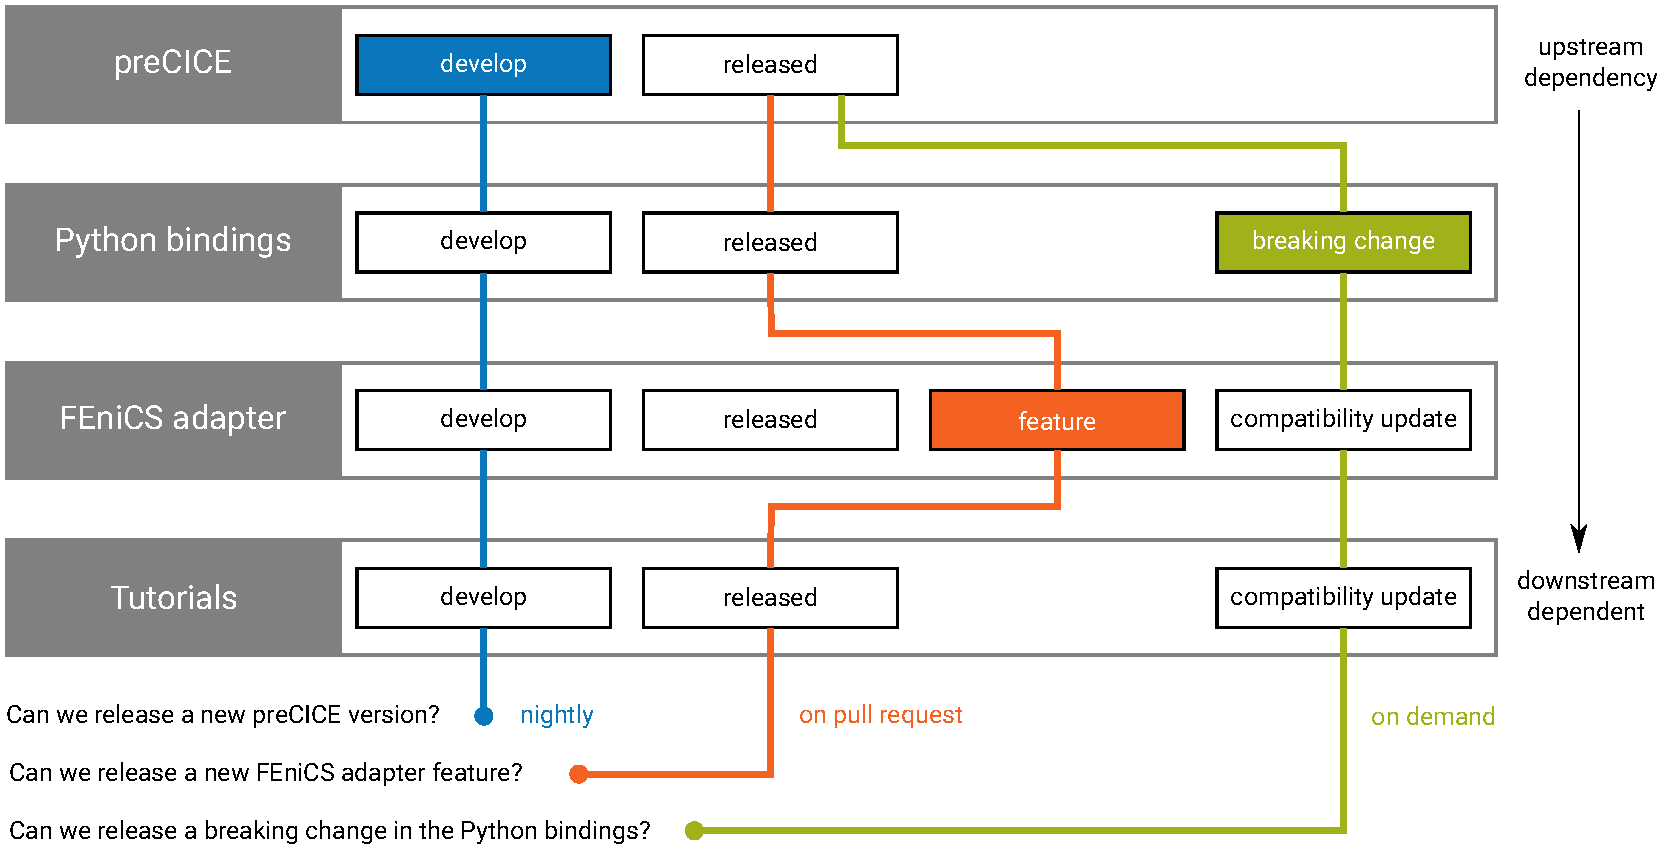
\includegraphics[width=\textwidth]{figs/tests-branches.pdf}
  \caption{Example questions that the system (regression) tests of preCICE help us answer (planned workflow).
  The system tests are always executed at the bottom-most layer (tutorials repository), using Docker images prepared in the layers above.
  Every night, all develop branches are tested together, to ensure that a new version of preCICE can be released at any time (blue).
  Pull requests that introduce non-breaking changes are automatically tested against the latest released versions of the other repositories (orange).
  Pull requests that introduce breaking changes need additional coordination with downstream projects and the tests need to compose compatible branches (green).
  The Python bindings and the FEniCS adapter only serve here as examples; in practice, more repositories are involved.}
  \label{fig:tests-branches}
\end{figure}

As these tests take a long time to prepare and execute and as they are particularly challenging to log in a structured and effective way,
executing the complete test matrix is not realistic and we need to select representative configurations.

We restrict the test matrix to a set of strategically important combinations. In terms of platforms, we execute most tests on the platform most common among users, currently the latest Ubuntu LTS version. We also execute selected tests on the oldest supported platform (previous Ubuntu LTS) and on the latest state of the continuously-updated Arch Linux. In terms of branches, we test each proposed branch with the rest of the components in their latest released state: this helps Lisa, Adam, and Tudor develop their projects independently, without worrying about untested new features. In case a breaking change is introduced in one component, then this needs to be tested in combination with corresponding compatibility updates in the downstream components. We also test the development branches of all components together in nightly builds, so that Maria and every developer can confidently release new versions of each component.

Maintaining the system tests and reference data up-to-date requires significant effort and any failing tests need to be addressed quickly, so that they remain useful and trusted. We observed that deep understanding and documentation of known issues that trigger test failures is crucial for the infrastructure to facilitate instead of hinder the development. Similarly, easily accessible logging of different levels is very important to verify that all relevant tests have succeeded and to precisely identify any faults. Finally, even though the operations need to be automatic enough to get green lights at the right places, developers do want to be able to form a clear mental model of the system behind the automation in order to trust the system and try to debug it, if needed.

Since preCICE v1 and till v2.1, we maintained the system tests on a dedicated repository\footnote{preCICE system tests on GitHub: \url{https://github.com/precice/systemtests}} using Travis CI. This repository contained scripts to run tests, scripts to prepare the test cases, as well as reference data for each test case. Because of policy changes in Travis CI and increasing flexibility offered by newer alternatives, we phased-out this implementation and we have been migrating to a different system. We describe here the outdated architecture of the tests used for preCICE v2.1 and discuss issues and potential solutions.

With every new commit pushed to an adapter repository, the Travis CI instance of the adapter instructed the Travis CI instance of the \incode{systemtests} repository to run any tests (tutorials) it knew to involve this adapter. Travis CI then built Docker images of preCICE adapters and pushed these to Docker Hub so that they could be reused. It then started one Docker container per simulation participant, as well as one Docker container serving the tutorial configuration. We used Docker Compose to build connections between the containers and we set a commonly accessible directory to exchange necessary connection tokens for the inter-code communication, as described in \autoref{ssec:com}.
% \footnote{As preCICE can rely directly on the widely used TCP/IP protocol, this technique can also be used to construct partitioned simulations among different computers.}.

At the end of each test case, a script compared the results. We originally compared every available results file excluding lines unique to every run. To account for sporadic rounding errors, we filtered arithmetic data and applied a numerical comparison. As this approach was very tedious to maintain for every new solver, we switched to comparing only the exported VTK files of the preCICE interface meshes. With a common file format at hand, the comparison scripts became much easier to execute and maintain. We also found this simplification to be enough for identifying regressions in the coupling, which is our main interest.
After Travis CI compared the results, it archived key log files to a dedicated repository \incode{precice_st_output}.
% This was necessary, as the web interface could only display the linear terminal output, which was difficult to parse, especially in a partitioned simulation.
% The archived log files include a summary of the executed test (including the involved commits of every involved repository), the logs of each participant, and the logs of preCICE.
% To guide the user in this multi-project workflow, the \incode{systemtests} Travis CI job id was reported back to the
% adapter Travis CI log. In case of a failure, a developer needed to find this job id, inspect the related job, and look for more details in the \incode{precice_st_output} archive.
This was a far-from-ideal logging solution, leading to cumbersome workflows to discover more details about the executed tests and potential failures.

We are currently redesigning our system tests. Key decisions so far have been to separate the machinery from the reference data, hosting the (reduced) reference data together with the configurations that produce them (tutorials), so that they can be updated at the same time. More recent tools, such as GitHub Actions and GitLab CI, offer multi-project pipelines and more possibilities for storing artifacts and archiving logs. With such additional options to avoid complex workarounds and with our experience from the aforementioned approaches, a redesigning was deemed reasonable and is expected to fruit in the near future. Until then, we rely on regular manual runs with every release.

\subsection{Additional checks} 
\label{ssec:additional_checks}

To maintain the quality and consistency of the codebase, the preCICE CI runs additional checks on the latest state of every pull request.
The CI uses a fixed version of clang-format\footnote{clang-format: \url{https://clang.llvm.org/docs/ClangFormat.html}} to check all C++ and C files, as well as a custom formatter based on the Python lxml\footnote{lxml: \url{https://lxml.de/}} package to check all XML configuration files for correct formatting.
As most CI environments provide multiple CPUs, the system uses GNU parallel~\cite{gnuparallel} to leverage the available compute resources.

When building and testing on Ubuntu, the CI additionally generates the Debian packages using CPack\footnote{CPack: \url{https://cmake.org/cmake/help/latest/module/CPack.html}} and test them using the Debian package checker Lintian\footnote{Lintial: \url{https://wiki.debian.org/Lintian}}.
Furthermore, the tests generate code testing coverage information using GCC.
The resulting coverage information is then gathered by LCOV\footnote{LCOV: \url{http://ltp.sourceforge.net/coverage/lcov.php}} and uploaded to the Codecov\footnote{Codecov: \url{https://about.codecov.io/}} service, which integrates the coverage report into the GitHub user interface.
This informs the reviewer about the coverage of the code change, as well as the resulting coverage change of the whole project.

Moreover, the external code quality services lgtm\footnote{lgtm: \url{https://lgtm.com/}}, CodeFactor\footnote{CodeFactor: \url{https://www.codefactor.io/}}, and Codacy\footnote{Codacy: \url{https://www.codacy.com/}} are integrated into the core library's GitHub project and automatically run to perform code analyses using webhooks.
A scheduled job runs the proprietary static code analysis tool Coverity Scan\footnote{Coverity Scan: \url{https://scan.coverity.com/}} on the codebase once per week and reports the results to the developer mailing list.
These tools are useful to find less obvious issues such as code complexity, code duplication, misspellings as well as technical issues such as unreachable code, code paths leading to using uninitialized variables, incorrect exception handling, and more.

We use publicly available GitHub Actions from the marketplace\footnote{GitHub Actions Marketplace: \url{https://github.com/marketplace?type=actions}} to apply such checks on less critical components:
we validate shell scripts using shellcheck\footnote{shellcheck: \url{https://github.com/koalaman/shellcheck}, via GitHub Action \incode{ludeeus/action-shellcheck}},
we validate and format Python scripts using autopep8\footnote{autopep8: \url{https://github.com/hhatto/autopep8}, via \incode{peter-evans/autopep8}},
we validate the syntax of our documentation files with markdownlint\footnote{markdown-lint: \url{https://github.com/DavidAnson/markdownlint}, via \incode{articulate/actions-markdownlint}},
and we check for broken hyperlinks using markdown-link-check\footnote{markdown-link-check: \url{https://github.com/tcort/markdown-link-check},\\ via \incode{gaurav-nelson/github-action-markdown-link-check}}.
Finally, we publish Python packages using twine\footnote{twine: \url{https://github.com/pypa/twine}}.

Code reviews provide an additional safety check, which can prevent issues that are otherwise difficult to check automatically. Pull request templates provide checklists for authors and reviewers. Most non-trivial code contributions to preCICE since 2018 are reviewed by at least one further core developer. The master branches are protected from pushing and from merging without reviews.

Apart from tests and quality checks, a few more operations contribute to maintaining the resources available to the user up-to-date. A GitHub Actions workflow builds and packages a Vagrant\footnote{Vagrant: \url{https://www.vagrantup.com/}, see also~\autoref{ssec:building}.} box for VirtualBox with the latest Ubuntu LTS and all common components and tutorials pre-installed. A similar workflow prepares and publishes Docker images with all the preCICE dependencies, images which we use for our CI\footnote{preCICE CI images: \url{https://github.com/precice/ci-images}, Docker: \url{https://hub.docker.com/u/precice}}. The website of preCICE is also automatically generated using GitHub Pages\footnote{preCICE Website sources: \url{https://github.com/precice/precice.github.io}}, integrating content from additional repositories (tutorials and adapters). Finally, a dedicated workflow periodically updates the Doxygen-based C++ source documentation.
